Um sistema de aquisição de dados, ou DAQ do inglês \emph{Data Acquisition Systems}, é um dispositivo, ou um conjunto deles, capaz de coletar, armazenar e distribuir uma determinada informação de tal forma que esta, posteriormente, possa ser manipulada ou utilizada para entender melhor o fenômeno. Na prática esses sistemas são utilizados para capturar dados de uma determinada variável física de um processo, geralmente vinda de um sensor.

Inicialmente os sistemas de aquisição de dados eram dispositivos eletromecânicos que mostravam uma determinada grandeza física em um visor analógico e registravam as mesmas em papeis ou fita magnéticas, estes primeiros aparelhos que registrava dados de maneira independente ficaram conhecido como {Data Loggers}. Atualmente o uso de {Data Loggers} ainda é bastante comum, por serem sistemas simples e robustos, entretanto, com o avanço da eletrônica e com o advento dos computadores surgiram novas classes de aparelhos que capturam dados, dentre eles os que podem ser conectados a PCs e trabalham em conjunto com software como MATLAB e LabVIEW, esta classe de dispositivo é conhecida como \emph{PC-based data acquisition equipament}, ou em português, equipamentos de aquisição de dados para computadores \cite{daqbook}.

Os primeiros DAQs que se comunicava com computadores surgiram na década de 60 inicialmente utilizado pelas grandes industrias e centros de pesquisa, entretanto, a partir da década de 90, com a popularização dos computadores pessoais surgiram os primeiros DAQs na forma de placas de extensão para computadores utilizando os slots de extensão PCI, as chamadas \emph{plugin-in cards}. Hoje em dia os \emph{slots} PCIs evoluiram para o padrão \emph{PCI-express}, um barramento com elevadíssima taxa de transmissão de dados, podendo chegar a até 32GB/s para o padrão \emph{PCI-express 4.0}, ou PCI-E \cite{tecmundopcie}, as placas PCI ainda existem, mas estão entrando em desuso pois todas as placas-mãe atuais vêm de fábrica com o novo padrão. Na figura \ref{figura:pcixpcieni} tem-se dois modelos de DAQs na forma de placa de extensão de computadores com o padrão PCI (Esquerda) e o padrão PCI-Express (Direita).

\begin{figure}
	\centering
	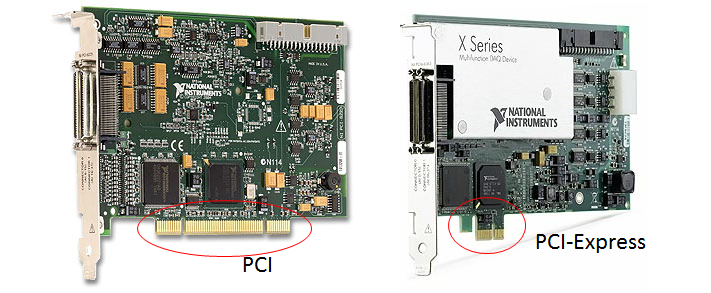
\includegraphics[width=0.8\textwidth]{figuras/pcivspcienational.png}
	\caption{Placas PCI e PCI-Express da National Instruments. \cite{lojanational}}
	\label{figura:pcixpcieni}
\end{figure}

Os modelos de DAQs na forma de extensão de placas para PCs foram bastante comuns na década de 90, porém esta classe de dispositivos podem sofrer interferência eletromagnética e eletrostática devido as máquinas rotativas dos computadores, como os \emph{coolers} e a própria estrutura de barramentos do computador, necessitando de um sistema de proteção contra este tipo de interferência. Atualmente os fabricantes vem disponibilizando sistema de aquisição de dados em uma caixa separada do computador garantindo um isolamento melhor em relação as interferências do computador. O fato de está externo ao computador, permite, também, uma maior mobilidade e menos restrição de espaço podendo ser utilizado em conjunto com \emph{notebooks}, não se limitando apenas a uma máquina, e ainda, em alguns casos, permitindo a comunicação entre DAQs a metros ou quilômetros de distância e o computador. 

Estes dispositivos isolados do computador só foram possíveis porque a comunicação entre o PC e seus periféricos externos evoluiu bastante. Os primeiros dispositivos isolados, ou \emph{stand-alone}, utilizavam principalmente a comunicação serial, RS232 e suas variantes como o RS485, para o caso do meio industrial. Estes padrões ainda são bastante comum no meio industrial e entre dispositivos embarcados, porém, não permite altas taxas de transferência, daí a preferência por placas PCI no passado. Com o surgimento de protocolos de comunicação mais recentes, como a USB, à partir da versão 2.0 e a \emph{Ethernet}, incluindo, mais recentemente, as redes sem fio, os DAQs \emph{stand-alone} com vários canais de alta velocidade, no qual necessita de um tráfego intenso de dados, se tornaram viáveis.

Historicamente os sistemas de aquisição de dados foram criados para atender a necessidade de grandes industrias e centros de pesquisa. Estes tipos de equipamentos, por sua vez, nunca foram baratos, devido a necessidade de equipamentos de alta qualidade, principalmente, devido ao grande poder de compra dos clientes. Por isso, os maiores fabricantes dessa classe de dispositivos possuem soluções com preços pouco convidativos, e quase sempre atrelados a \emph{software} e \emph{hardware} proprietário. Para exemplificar, a \emph{National Instruments} (NI), uma grande fabricante no ramo, vendem DAQs que variam de R\$ 2.087,88 a R\$ 63,540, segundo a loja oficial no Brasil \cite{lojanational}. O uso de \emph{software} e \emph{hardware} proprietários torna comum a prática de venda casada, pois para o funcionamento completo do DAQ é necessário adquirir mais de um produto, um anuncio da DAQ Instruments de um pacote incluindo o DAQ e os softwares necessários para o seu funcionamento exemplifica esta prática. Sozinho o aparelho custa \$59,00, porém, para ter a melhor experiência o fabricante sugere a compra de um pacote de \$244,00 (Figura \ref{figura:vendacasada}).

\begin{figure}
	\centering
	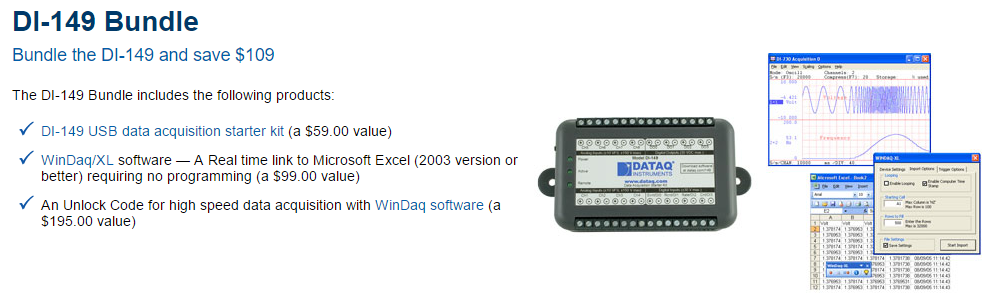
\includegraphics[width=0.9\textwidth]{figuras/bundle.PNG}
	\caption{Exemplo de anúncio de venda casada do Kit DI-149. \cite{dataqcasada}}
	\label{figura:vendacasada}
\end{figure} 

Na topologia padrão de um DAQ conectado a um computador é necessário converter o sinal analógico, geralmente vindo de um sensor, para dados digitais, de tal forma que possa ser reconhecido pelo computador. Esses dados posteriormente serão enviados através de uma interface de comunicação entre o computador e o DAQ. Para que tudo isso seja possível existe uma CPU capaz de gerenciar os dados de entrada conversor analógico digital, ou ADC (\emph{Analog-to-digital converter}), e a interface de comunicação. Um esquemático dessa topologia pode ser visto na figura \ref{figura:esquematico-daq-pc}.

\begin{figure}
	\centering
	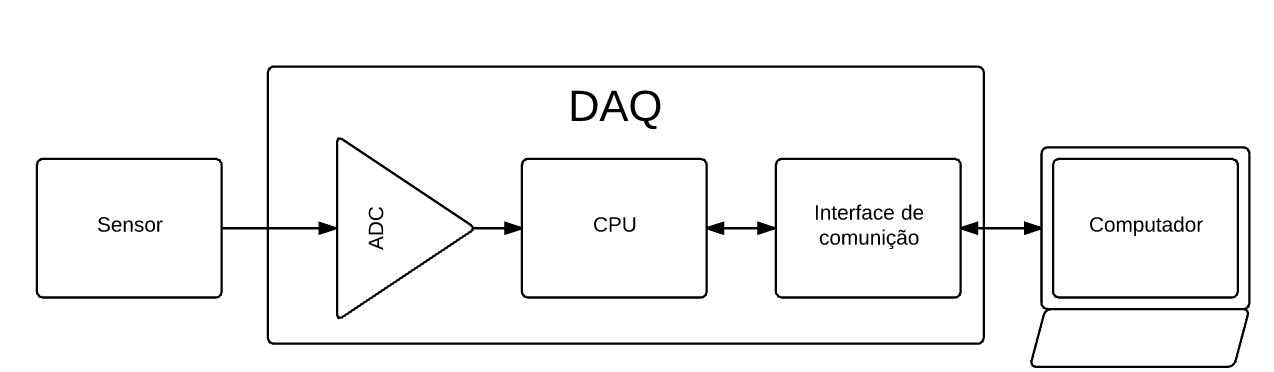
\includegraphics[width=0.9\textwidth]{figuras/daq-esquema.png}
	\caption{Esquemático de um DAQ conectado a um computador (Próprio Autor)}
	\label{figura:esquematico-daq-pc}
\end{figure}

Na verdade, a topologia do DAQ representado na figura \ref{figura:esquematico-daq-pc} é algo bastante comum na eletrônica embarcada, por isso, já vem embutida em alguns microcontroladores. Sistemas embarcados, são dispositivos feitos para um propósitos específico, desde ao controle de um elevador ao gerenciamento de um instrumento de aquisição de dados. Nestes sistemas é comum o uso de microcontroladores, que são computadores dedicados àquela tarefa exclusiva. Muitos microcontroladores, além da CPU e memória, vem com diversos protocolos de comunicação, ADCs, DACs (Digital Analog Converters) embutidos em um único encapsulamento. Essa integração de diversos periféricos em um único \emph{chip} deixa o projeto mais simples e barato, por isso é cada vez mais comum os fabricantes disponibilizarem sistemas cada vez mais completos em um único encapsulamento. Esse conceito é conhecido como \emph{System on Chip}, os famosos SOCs, que estão embarcados nos mais diversos dispositivos, até mesmo em celulares.

Os primeiros microcontroladores surgiram no final do século passado. Inicialmente eles não eram muito acessíveis, tanto na questão de preço quando na complexidade de programação e desenvolvimento. Muito deles tinham que ser programados em \emph{Assembly}, ou linguagem de máquina, por causa da baixa memória disponível. Entretanto, com o tempo os novos modelos vieram com mais memória, mais poder de processamento e periféricos mais avançado, junto a isso, como tudo na tecnologia, surgiu novas ferramentas e compiladores, facilitando bastante o desenvolvimento de dispositivos microcontrolados. Uma grande evolução nesse sentido aconteceu em 2005, quando um grupo de pesquisadores da Itália propuseram uma plataforma de prototipagem de baixo custo, fácil utilização e de código aberto, conhecida como Arduino. O \emph{hardware} do Arduino é uma placa de desenvolvimento completa, ou seja, além do microcontrolador, ela vem com todos os circuitos externos para o seu funcionamento, incluindo fonte de alimentação, regulador de tensão, oscilador externo, entrada USB e pinos de extensão \cite{tedarduino}. Além do \emph{hardware} pronto para o uso o Arduino dispõe uma linguagem de programação que abstrai os elementos de \emph{hardware} do microcontrolador, portanto é possível programar no Arduino sem precisar setar nenhum valor em registradores do microcontrolador, as bibliotecas e funções disponível na linguagem já faz todas as configurações necessárias para o usuário leigo. O fato de ser código aberto e a facilidade de utilização atraiu diversos entusiastas, hobbistas e profissionais para a plataforma, se tornando uma das maiores comunidades, se não a maior, de sistemas embarcados atualmente. 

De uma forma geral, o Arduino, além de aumentar o número de pessoas interessadas em eletrônica, aumentou a quantidade de projetos e velocidade com que eles eram feitos, possibilitando a criação de projetos como tênis que amarra sozinho e impressoras 3D \cite{tenissozinho}. Hoje existem diversos fabricantes que fabricam módulos de expansão para o Arduino conhecidos como Shields. Existem módulos para tudo, controle de motores, relés, conexão \emph{ethernet} e Wi-Fi, \emph{bluetooth}, dentre outros. Com os módulos o usuário só precisa comprar conectores e programar, não havendo a necessidade de criar circuitos complexos na \emph{protoboard} ou fazer placas de circuito impresso.

Depois que o Arduino se tornou popular diversas organizações e empresas resolveram criar suas placas de desenvolvimento \emph{open source}. Na época em que o Arduino foi criado surgiram os primeiros \emph{smartphones}, junto com eles, os SOCs com processadores ARM e GPUs de baixo consumo que permitiu aliar o baixo consumo, dissipação de calor, tamanho portátil e alto desempenho em um único \emph{chip}. Em 2008 a Texas Instruments, uma empresa privada que desenvolve diversos produtos semicondutores como microcontroladores e SOCs com arquitetura ARM para celulares, resolveu criar a Beagleboard em parceria com a Digikey e a Element14, duas empresas do ramo de varejo eletrônico nos EUA. A ideia era demonstrar o poder do SOC  OMAP3530 em uma placa de desenvolvimento do tamanho de cartão de crédito, capaz de rodar uma distribuição Linux portada para ARM incluindo os aplicativos compilado este sistema operacional.  A ideia foi promissora, pois foi uma das pioneiras na área de computadores embarcados, mas o preço de \$125 não fez a placa decolar. O Linux embarcado, ou E-Linux, só se tornou popular quando a fundação Raspberry Pi resolveu criar um produto de mesmo nome por apenas 35 dólares, em fevereiro de 2012. A ideia da fundação era criar uma plataforma de programação de baixíssimo custo \cite{tecmundopi}. Hoje Raspeberry Pi é de longe a \emph{E-Linux board} mais vendida e com a maior comunidade. \emph{E-Linux boards} é o termo utilizado para computadores que rodam linux embarcado.

Junto ao sucesso do Raspberry Pi, surgiram diversas outras opções de empresas e fundações que queria por sua plataforma \emph{open source} com Linux embarcado no mercado, ou atualizá-las como foi o caso da empresa criadora do Beagleboard. Assim aproveitando a onda dos computadores \emph{single board} a Texas Instruments criou o BeagleBone Black. O grande diferencial deste computador em relação ao Raspberry Pi à Beagleboard está nos periféricos. O BBB (Abreviação de Beaglebone Black) tem 65 pinos de extensão, um microcontrolador auxiliar para programação em tempo real, o PRU, e muito mais periféricos que o Raspberry Pi. Para efeito de comparação na tabela \ref{tab:compsingleboardpcs} tem-se o comparitivo entre o Beaglebone Black, Arduino Yun, uma das versões do arduino com Linux embarcado, e o Raspeberry Pi. Pela tabela percebe-se que o BBB é o único concorrente que alia o alto poder de processamento com a grande quantidade de periféricos e I/O, termo inglês para representar os pinos de extensão de entrada, \emph{input}, e saída, \emph{output}. A quantidade elevada de I/Os permitiu a fabricante do Beaglebone criar o conceito de placas de expansão para a \emph{E-Linux board} conhecida como Capes, semelhante aos Shields disponíveis para Arduino. 
	
\begin{table}
	\centering
	\begin{tabular}[c]{c|ccc}
		&Arduino Yun&Beaglebone Black&Raspberry Pi\\ \hline
		CPU&MIPS32&ARM Cortex-A8&ARM1176\\
		CPU Freq.&400Mhz&1Ghz&700Mhz\\ 
		Microcontrolador&ATmega32U4&PRU&Não tem\\ 
		\(\displaystyle \mu \)controlador Freq.&16Mhz&200Mhz&-\\
		RAM&64Mb&512Mb&512Mb\\ 
		GPU&Não tem&PowerVR SGX530&Broadcom VideoCore IV\\ 
		Memória interna&16Mb&4GB&Não tem\\ 
		Memória externa&Micro SD&Micro SD&SD\\ 
		I/O&20&65&17\\
		Ethernet&10/100 Mbit&10/100 Mbit&10/100 Mbit\\ 
		ADC&12x 10bits, 0-5V&7x 12bits 0-1.8V&Não tem\\ 
		PWM&7x&8x&1x\\ 
		UART&2x&4x&1x\\ 
		SPI&1x&2x&2x\\ 
		I2C&1x&2x&1x\\ 
		USB \emph{Host}&1x&1x&2x\\
		USB \emph{Client}&1x&1x&Não tem\\ 
		Video&Não tem&Micro HDMI&HDMI, RCA, DSI\\ 
		Audio&Não tem&Micro HDMI&HDMI, P2\\
		Preço&\$75&\$55&\$35\\ \hline
	\end{tabular}
	\caption{Comparação entre os \emph{E-linux board} \emph{open source} mais usados no mercado \cite{comparisonelinux}.}
	\label{tab:compsingleboardpcs}
\end{table}
	
O Beaglebone Black quando foi lançado fez um relativo sucesso, mais que o seu antecessor, principalmente pela nova política de preço, seu microcontrolador integrado e a quantidade generosa de I/Os e periféricos. Entretanto isso não foi o suficiente para desbancar o Raspberry Pi. Parte disso é devido a forma de como as \emph{E-Linux boards} são utilizadas. A maioria das aplicações desses \emph{single board computers} está na área de computação, como na criação de pequenos servidores, centrais de emulação, \emph{media centers}, câmeras de vigilância, dentre outros. Para isso, as poucas portas e periféricos do Raspberry Pi é o suficiente. Quando há a necessidade de alguma aplicação em tempo real geralmente utiliza-se o Raspberry Pi em conjunto com o Arduino. O outro motivo para o Beaglebone não ter desbancado o Raspberry Pi, foi o fato de este último ter sido lançado muito tarde. Em 2013, quando foi lançado, a comunidade do Pi já estava grande e já existiam outros concorrentes, como a Cubie Board. Além disso, as Capes que poderiam ser um grande diferencial são muito caras e não há muita variedade. Na prática o BBB é uma dos \emph{sigle board computers} mais utilizados, mas está longe de ser a mais popular e o conceito de Capes não engrenou como a fabricante previa.
	
Embora Beaglebone Black tenha todos esses contras, ele ainda é a melhor opção de \emph{E-Linux computer} para a construção de um DAQ. Pois para a criação de um DAQ é necessário um ADC de boa qualidade, uma CPU de alto desempenho para processar todos os dados capturados e interfaces de comunicação de alta velocidade, como Ethernet e USB 2.0. Por isso este trabalho pretende utilizar o Beaglebone Black para criar um sistema de aquisição de dados de baixo custo conectado ao computador pela porta USB. Sistema no qual será utilizado posteriormente para a captura de dados de um acelerômetro analógico industrial, em trabalhos futuros.
